\documentclass{scrartcl}
\usepackage{style}
% version
\newcommand{\versionmajor}{0}
\newcommand{\versionminor}{1}
\newcommand{\versionpatch}{0}
\newcommand{\version}{\versionmajor.\versionminor.\versionpatch}

\title{\LARGE
    ChainVote Final Report
}

\subtitle{(v. \version)}

\author{
    Giovanni Antonioni \\ \emailaddr{author1@email.it}
    \and 
    Luca Rubboli \\ \emailaddr{author2@gmail.com} 
    \and 
    Luca Tassinari \\ \emailaddr{luca.tassinari10@studio.unibo.it}
}

\date{\today}

\begin{document}

\maketitle

\begin{abstract}
    Electronic voting systems based on blockchain technology have emerged as a potential solution to enhance the security and transparency of traditional voting methods. In this system, voters cast their votes electronically, and the results are stored on a decentralized blockchain ledger, which ensures the integrity of the vote by preventing any tampering or manipulation. This system provides a transparent and immutable record of votes, which can be accessed by anyone in the network, thus increasing trust in the electoral process. Nevertheless, the use of blockchain technology in electronic voting systems holds promise for creating a more secure, transparent, and democratic electoral process.

    This project aims to... \todo{finish}
\end{abstract}

\section{Goals/requirements}

\desc{
    Detailed description of the project goals, requirements, and expected outcomes.
    %
    Use case Diagrams, examples, or Q/A simulations are welcome.
}

The project consists of the implementation of a small-scale distributed electronic voting system based on blockchain technology.
%
Specifically, the goal is to create a web application where users can authenticate and interact with votes, as described in the use scenarios presented below.
%
\todo{improve description}

\subsection*{Functional requirements}

Two main actors can be identified in the system: the \textbf{administrator}, taking care to create new votes, and the \textbf{user}, which interacts with them.

\begin{itemize}
    \item System administrators can create new votes that all users can participate in;
    \item System administrators can't cast a vote;
    \item Users must be able to register and authenticate to the system;
    \item A user is able to cast a vote up to once per ballot;
    \item A ballot is a set of mutually exclusive choices with a time limit that cannot be changed;
    \item While a vote is in "open" state, users are able to see only the turnout;
    \item Once an election is finished, all users (voters and abstainers) and administrators can
    see the results;
    \item Multiple elections can be in "open" state simultaneously.
\end{itemize}

\subsection*{Non-functional requirements}

\begin{itemize}
    \item The connection between a user and his vote must be hidden;
    \item security \todo{to complete}
\end{itemize}

\subsection{Scenarios}

\desc{
    Informal description of the ways users are expected to interact with your project.
    %
    It should describe \emph{how} and \emph{why} a user should use / interact with the system.
}

In \cref{fig:use-cases-diagram} are reported the main use cases that emerged from the requirements analysis...

\begin{figure}
    \centering
    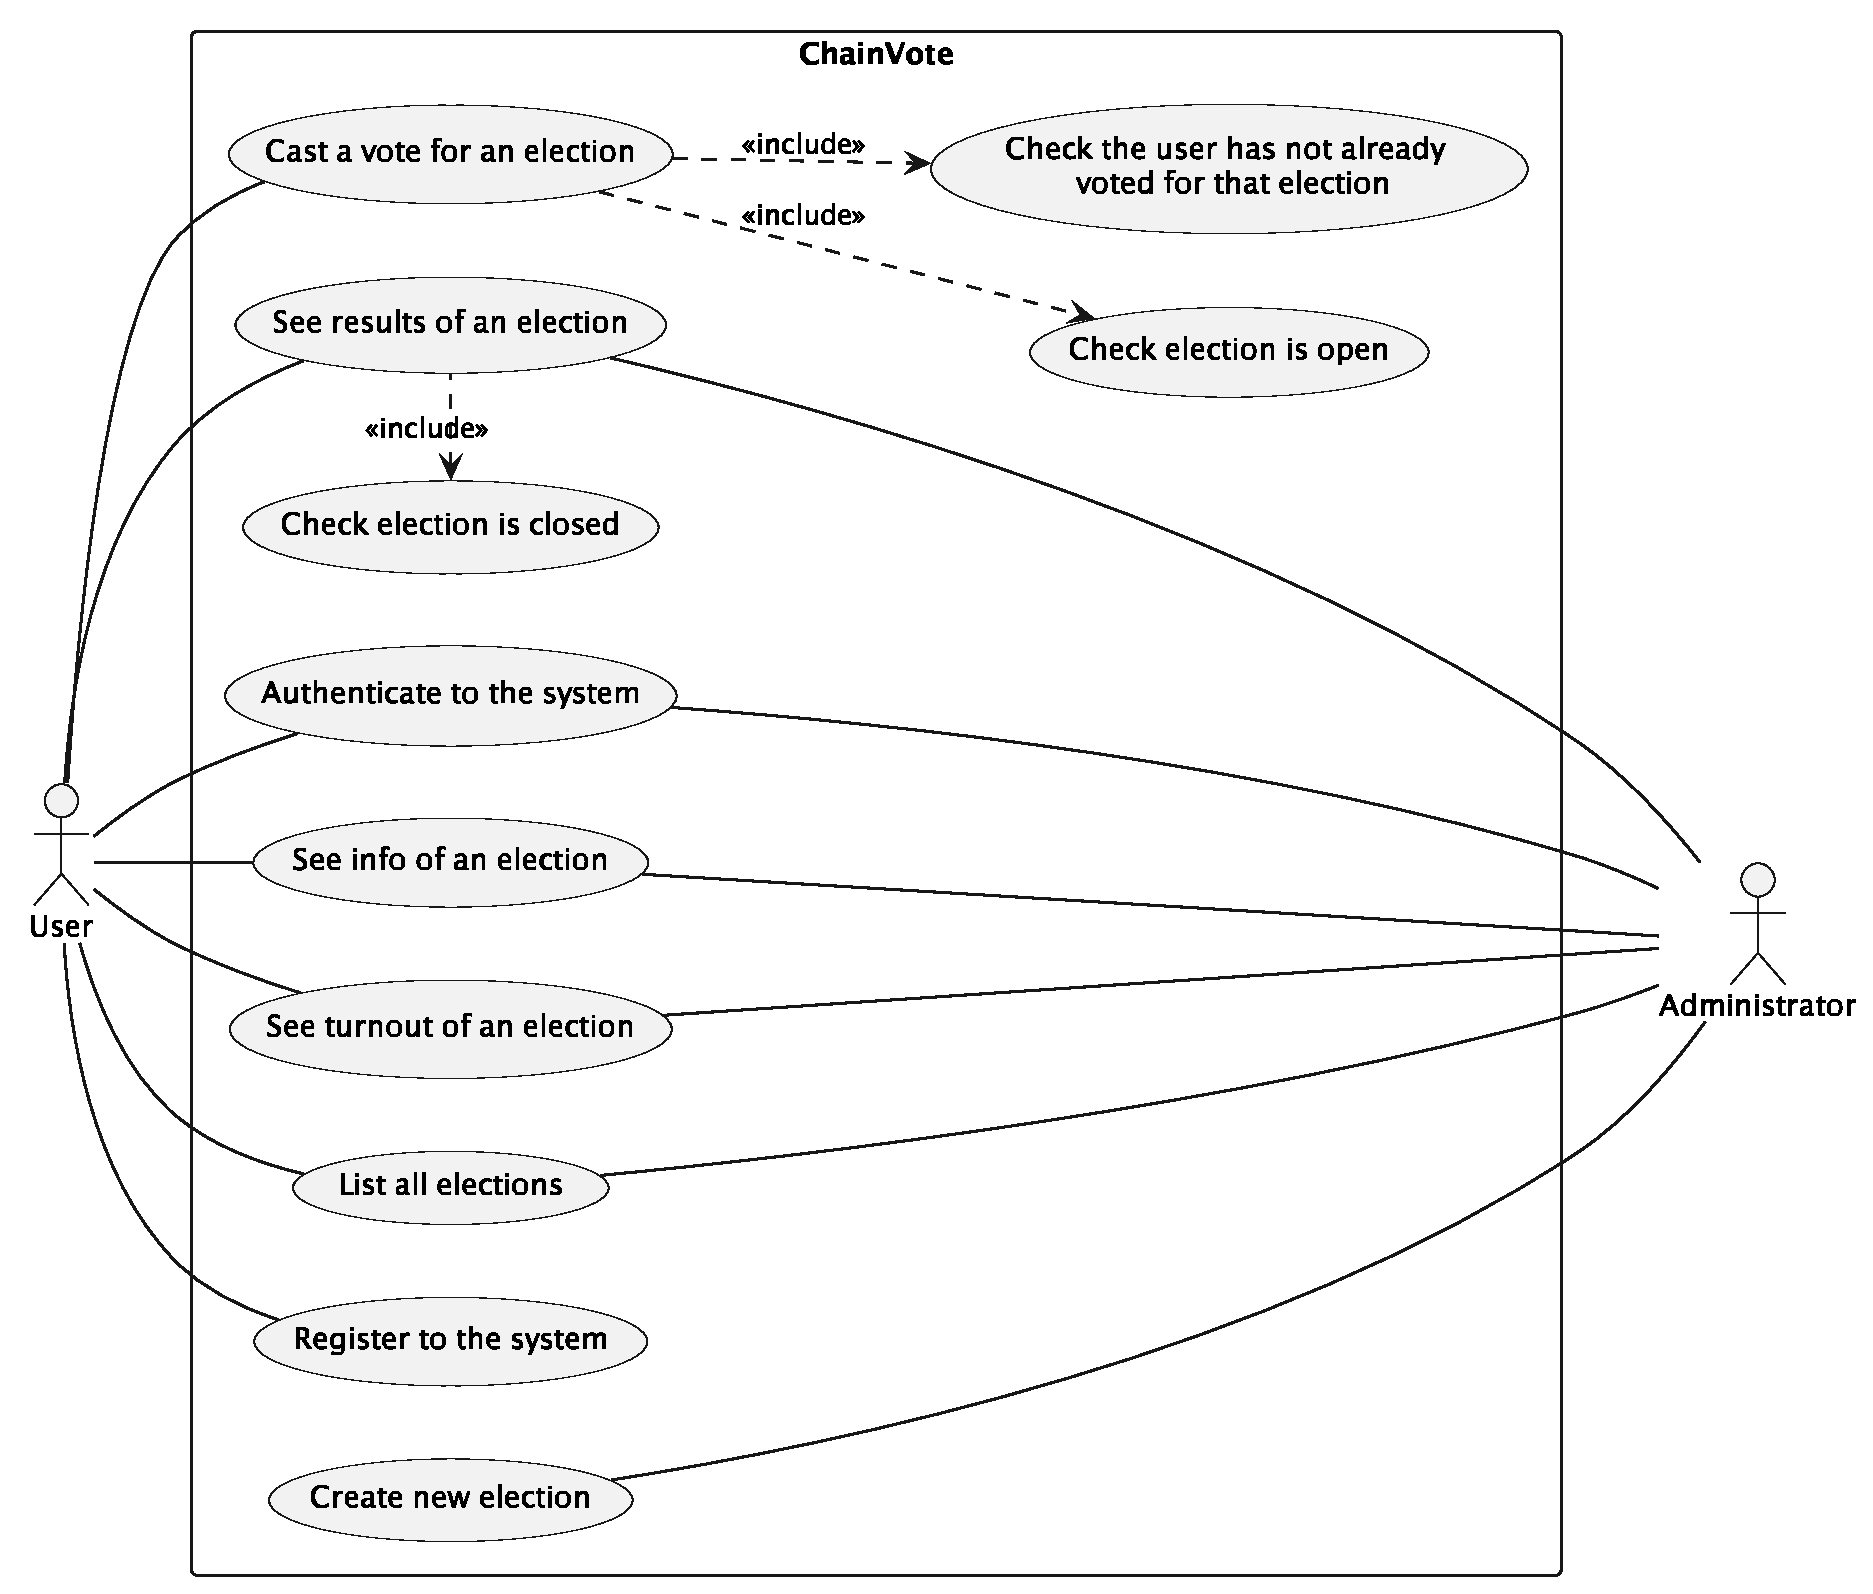
\includegraphics[width=\linewidth]{figures/use-cases.eps}
    \caption{Use cases of the ChainVote application identified as a result of the requirements analysis.}
    \label{fig:use-cases-diagram} 
\end{figure}

\subsection{Self-assessment policy}

\begin{itemize}
    \item How should the \emph{quality} of the \emph{produced software} be assessed?
    
    \item How should the \emph{effectiveness} of the project outcomes be assessed?
\end{itemize}

\section{Background}

Any preliminary notion necessary to understand the goals, the motivations, the context, or the development of this project.
%
\begin{itemize}
    \item Theoretical aspects
    
    \item Used frameworks / models / technologies (and motivation for their choice)
\end{itemize}

\section{Requirements Analysis}

Is there any implicit requirement hidden within this project's requirements?
%
Is there any implicit hypothesis hidden within this project's requirements?
%
Are there any non-functional requirements implied by this project's requirements?

What model / paradigm / techonology is the best suited to face this project's requirements?
%
What's the abstraction gap among the available models / paradigms / techonologies and the problem to be solved?

\section{Design}

This is where the logical / abstract contribution of the project is presented.

Notice that, when describing a software project, three dimensions need to be taken into account: structure, behaviour, and interaction.

Always remember to report \textbf{why} a particular design has been chosen.
Reporting wrong design choices which has been evalued during the design phase is welcome too.

\subsection{Structure / Domain Entities}

Which entities need to by modelled to reflect the domain?
%
(UML Class diagram)

How should entities be modularised?
%
(UML Component / Package / Deployment Diagrams)

\subsection{Behaviour}

How should each entity behave?
%
(UML State diagram or Activity Diagram)

\subsection{Interaction}

How should entities interact with each other?
%
(UML Sequence Diagram)

\section{Implementation Details}

Just report interesting / non-trivial / non-obvious implementation details.

This section is expected to be short in case some documentation (e.g. Javadoc or Swagger Spec) has been produced for the software artefacts.
%
This this case, the produced documentation should be referenced here.

\section{Self-assessment / Validation}

Choose a criterion for the evaluation of the produced software and \textbf{its compliance to the requirements above}.

Pseudo-formal or formal criteria are preferred.

In case of a test-driven development, describe tests here and possibly report the amount of passing tests, the total amount of tests and, possibly, the test coverage.

\section{Deployment Instructions}

Explain here how to install and launch the produced software artefacts.
%
Assume the softaware must be installed on a totally virgin environment.
%
So, report \textbf{any} configuration step.

Gradle and Docker may be useful here to ensure the deployment and launch processes to be easy.

\section{Usage Examples}

Show how to use the produced software artefacts.

Ideally, there should be at least one example for each scenario proposed above.

\section{Conclusions}

Recap what you did

\subsection{Future Works}

Recap what you did \emph{not}

\subsection{What did we learned}

Racap what did you learned

\section*{Stylistic Notes}

Use a uniform style, especially when writing formal stuff: $X$, X, $\mathbf{X}$, $\mathcal{X}$, \texttt{X} are all different symbols possibly referring to different entities. 

This is a very short paragraph.

This is a longer paragraph (notice the blank line in the code).
It composed by several sentences.
%
You're invited to use comments within \texttt{.tex} source files to separate sentences composing the same paragraph.

Paragraph should be logically atomic: a subordinate sentence from one paragraph should always refer to another sentence from within the same paragraph.

The first line of a paragraph is usually indented.
%
This is intended: it is the way \LaTeX{} lets the reader know a new paragraph is beginning.

\begin{figure} % DO NOT write any positional hint (e.g. [h] or [t] here!
    \centering
    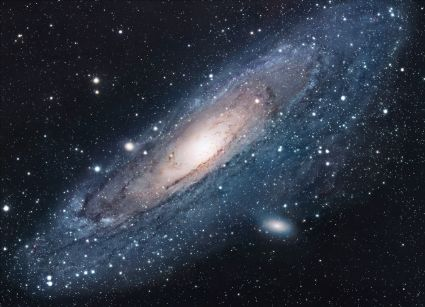
\includegraphics[width=0.5\linewidth]{figures/universe.jpg}
    \caption{Some floating image}
    \label{fig:image} 
\end{figure}

Let \LaTeX{} decide where to put figures (or tables, or listings), label them and reference the labels instead of say things like ``in the following image...''.
%
Consider for instance the case of \cref{fig:image}.

Use the \href{https://en.wikibooks.org/wiki/LaTeX/Source_Code_Listings}{\texttt{listing}} package for inserting scripts into the \LaTeX{} source.
%
Consider for instance \cref{lst:snippet}.

% have a look to macros in code-listings.sty
\javaimport[
    caption={Some Java listing},
    label={lst:snippet}
]{listings/HelloWorld.java}

\nocite{*} % Includes all references from the `references.bib` file
\bibliographystyle{plain}
\bibliography{references}

\end{document}
